\documentclass[12pt]{article}
\title{Forklift Frenzy Group Report}
\author{Alexander Haining 40283659\\David MacGruer 40172073\\Matias Nilla Matias Rafael Malmivaara 40286188\\Matthew Newbigging 09004805\\Marie Pearson 40181382\\Zoe Wall 40182161}
\date{\today}
\usepackage{graphicx}
\usepackage{float}
\usepackage{pdfpages}
\usepackage{titlesec}
\usepackage[a4paper,outer=1.5cm,inner=1.5cm,top=1.75cm,bottom=1.5cm]{geometry}
\setcounter{secnumdepth}{2}

\newcommand{\figuremacro}[5]{
	\begin{figure}[#1]
		\centering
		\includegraphics[width=#5\columnwidth]{images/#2}
		\caption[#3]{\textbf{#3}#4}
		\label{fig:#2}
	\end{figure}
}

\begin{document}
\maketitle

\pagenumbering{gobble}

\newpage
\tableofcontents
\newpage
\pagenumbering{arabic}

\section{Abstract}
	This report details the progress made in completing the Forklift Frenzy group project, illustrates the various learning outcomes achieved and compares original aims with resulting deliverables.
		
	Forklift Frenzy is a 3D video game for use on Windows PC, suitable for an audience of all ages, created from original assets only. The game lets players take command of a number of various forklifts, with which they must navigate a map to retrieve and deliver certain packages for points, against the clock.
	
	The Group Project module provides the perfect opportunity to allow a group of students keen to work on games in their future careers to create a portfolio piece, whilst gaining some insight and experience in working in a small team to publish a game created from scratch. As such, Forklift Frenzy is a student led project, with the project manager acting as client. The roles and outcomes carried out by group members include:
	\begin{itemize}
		\item Project Manager, client and programmer - successful management of the software project; documentation, risk mitigation, feature definition, minor development tasks
		\item Lead Programmer - all major development tasks, version control
		\item Artists - asset creation to specifications; 2D concept and UI
		art, 3D models, textures, adhering to agreed asset standardisations
		\item Sound Designer - creating and implementation of all sound effects
	\end{itemize}
	
	Described in detail further on in this document, the success of the project relied on overcoming several key obstacles:
	\begin{itemize}
		\item Agreeing on a work pipeline suitable to create usable game ready assets
		\item Appropriate collaboration in having multiple artists and programmers work on similar tasks and the resolution of any conflicts 
		\item Thorough understanding of technologies used
	\end{itemize}
	
	The main deliverable for the project is the executable for the game itself, showcasing the work done by all team members as outlined above.

\section{Background}
Having an interest in working in the games industry, yet no real experience in doing so, this module seemed the perfect opportunity to do just that. Before the module began, last term, emails were sent to certain lecturers looking for recommendations of students who, while adept in their field, also possessed a similar interest to work in the games industry. Following brief interviews, the team was formed in which each member wished to use the module as an opportunity to create a portfolio piece. As such, the main aim of the project is to make available a playable game which demonstrates each team member’s proficiency in their field; game models and textures from the artists, original sound effects from the sound designer, game logic from the programmers and the successful handling of a software focused project by the project manager. 

Second to illustrating team members individual skills, another important learning outcome of this project is to demonstrate the ability to work together effectively, with those of different disciplines within the team, to have the project meet with success. Meeting this aim should result in a better understanding of an individual’s place in a group, and in putting systems in place to allow better collaboration and work flow between everyone involved.


\subsection{Context}
Forklift Frenzy is best put in context by considering its main purpose; a portfolio piece, rather than a means of making money. This software, while it will be used by the public, is not purposed to solve a particular problem, or have any use other than entertainment. It is not absolutely essential that the software runs bug-free, though it is of course preferred.


\subsection{Scope}
The scope of the project is such that only one operating system, Windows PC, will be targeted due to a focus on content and not compatibility across multiple platforms. The game itself will only include one playable level, the benefit of which is to require a minimal number of assets before the project may be called a success. This is largely due to the fact that game-ready assets take time to create, thereby limiting the number of assets that may be included given the short project time frame. The deliverable is intended to be a demo, or proof of concept, rather than a fully fledged game. 


\subsection{Limitations}
Time available is a considerable limitation to the project, the lack of which resulted in the original project goals being revised midway through the module. Lasting only one semester, and running alongside two other equally demanding modules, each member’s available time is never guaranteed to be the same every week throughout the project. This affects the number of tasks that may be completed throughout the project, meaning that the list of features that must be implemented before project end has to be concise, and monitored throughout to ensure that there is indeed adequate time to complete them.

A close second in terms of limitations is software experience, which impacts on time; many team members were interacting with the software used for the first time, resulting in a longer development cycle than might be thought of as typical for this sort of software project. Whilst each team member is proficient in their own field, there was at project start less overall experience in collaboration; storing and sharing work, ensuring assets passed on are usable by programmers, maintaining appropriate communications. This results in more time being spent working out effective systems and standardisations, further limiting the amount of tasks completed.


\subsection{Aims}
The original aims of the project were to have the game feature:
\begin{itemize}
	\item Single Player; a game mode which can be played without an internet connection. Allows players to complete missions to earn in-game currency, which can be redeemed to buy other types of forklift.
	\item Multiplayer; a game mode requiring an internet connection, in which up to six players on two teams compete on the same map to collect as many boxes as they can, with the winners having the most boxes collected at the end of the round.
	\item Menu System; consisting of a main menu, pause menu and forklift selection screen, allowing users to navigate to different game modes, edit options and quit the game. 
	\item Game state persistence; via loading and saving local player data. This allows players to continue from where they left of in previous playthroughs, maintaining their high scores, currency and forklift unlocks.
	\item Four forklift classes; with distinct models and characteristics for each.
\end{itemize}

Further to the above points, at project start it was intended that the game be submitted to Steam Greenlight. This process involves publishing screenshots, videos and a description of the game to Steam for users to view. Users then have the chance to upvote, or downvote, the game depending on whether they would like to see the game in the store to play for themselves. Should the game be the most voted at any time, Steam allow it to be published, and sold, through their store. 

\section{Results}
As mentioned previously, a chief goal of the project was to adopt an effective work flow between team members given the difference in disciplines present in the team; creatives, organiser and logical thinkers. The artists and sound designers were in charge of creating the assets that would appear in the game, while the programmers were responsible for building the logic and compiling the completed assets within the game scenes. This meant that tasks completed by the artists and sound designer flowed through the programmers, who also acted as testers. 

Underpinned by communication, the overall pipeline put in place allowed work to be shared across the team with relative ease; tasks were worked on individually, with team members being updated on progress or problems throughout the week. There were slight differences in the work flow for each discipline, as outlined below: 
\begin{itemize}
	\item Art: After being set the task of creating a certain model for the game, artists could work individually. On completion, the model was passed on to the lead programmer for integration into Unity, where it was also tested to ensure acceptance criteria was met, which includes meeting the agreed upon standards. Should any criteria not be met, the model would be sent back to be updated. 
	\item Programming: The numerous scripts necessary to create the game logic were developed in a certain order based on the scenes as they were made in Unity. Programmers would work on separate scenes where possible to make merging work simpler. Completed tasks would be first tested in Unity before a pull request was made to update the master branch with the latest work. 
	\item Sound: The sound designer was able to work individually for the most part; recording and editing sound clips formed a large part of the sound development cycle. Once the sound banks were made, the implementation required a programmer to edit existing code in order to add sound into the game. 
\end{itemize}



\subsection{Summary of Changes}
Given that the development time of certain assets, and completion time of some tasks, were uncertain at time of planning, extra time was allotted. Despite this, midway through the project it became clear that the original goals were too ambitious to complete before project end; there simply wasn't enough time to complete everything to standard. In order to ensure better quality and completeness in the final deliverable, a couple of goals were dropped from the project aims. (reflected in MSCW - put here or in PM?)

The first goal dropped was the multiplayer mode; this is a large undertaking in itself, and can be considered a separate game from single player due to numerous differences in game logic. It requires learning a different coding approach, networking, of which the time taken to achieve is uncertain.. At the time, there existed many bug related tasks to do with single player that were previously unaccounted for, so the decision was passed that multiplayer be dropped in favour of focusing on polishing the single player experience. (worth mentioning here that we said we'd work on it after project end, on our own time?)

Another goal set aside was the submission of the game to Steam Greenlight. Unfortunately, late in the project Steam announced that they would be replacing Greenlight with another, more costly alternative process. As such, this aim was dropped since the group did not wish to incur the cost to publish what is effectively a proof of concept rather than a full game.
 
\subsection{Outcomes}
With regard to each of the above outlined aims, this section compares the results achieved as seen in the final game. 
\subsubsection{Single Player Mode}
The vast majority of the work done throughout the project was put into the single player mode; most assets, sound clips and scripts created are showcased in this scene.
\begin{figure}[H]
	\caption{Single Player Screenshots}
	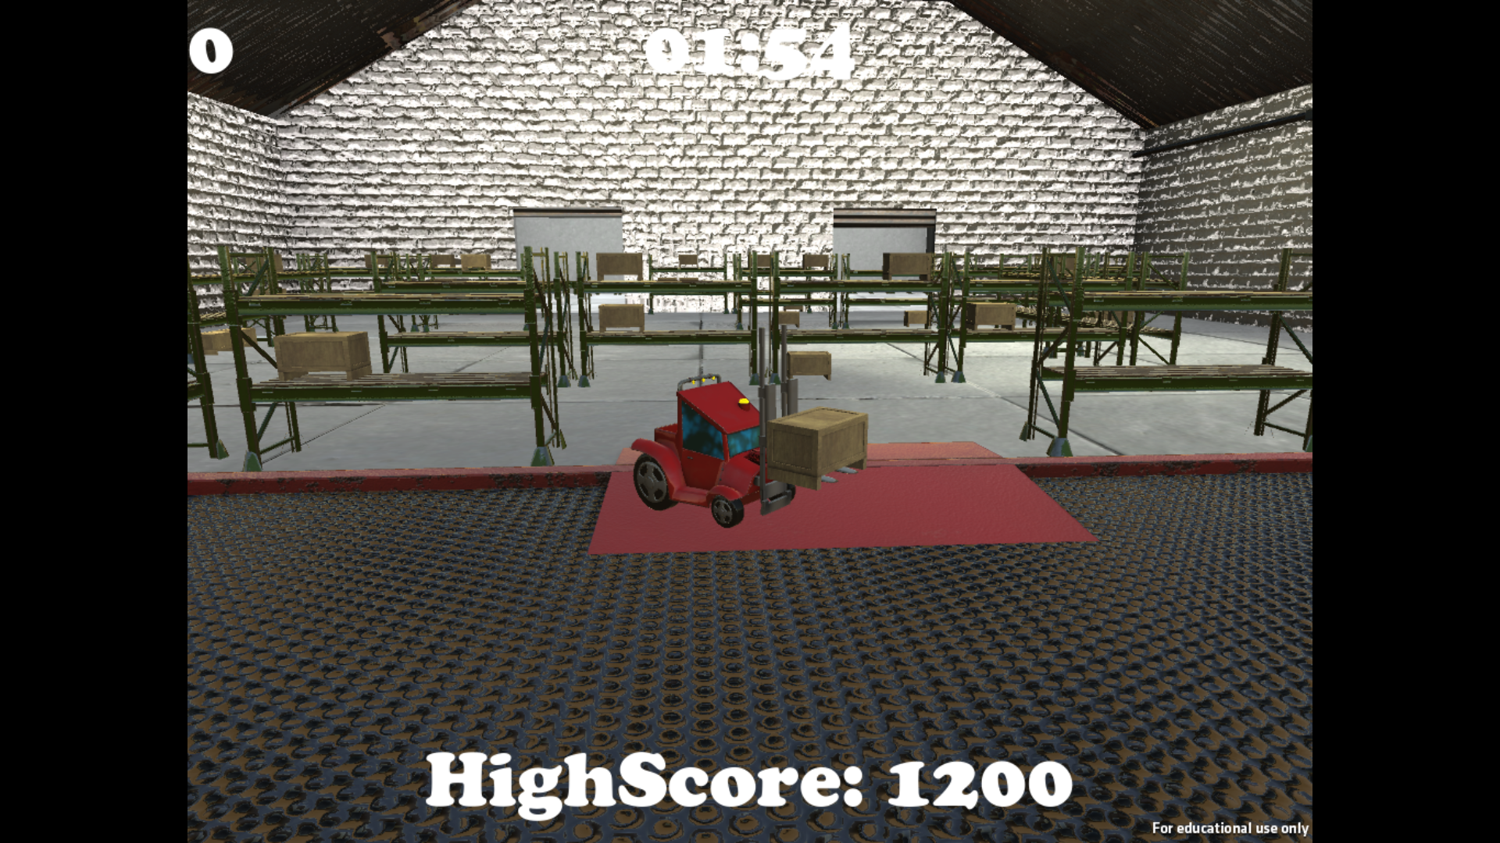
\includegraphics[width=\textwidth]{images/sp}
\end{figure}
This image was taken during single player gameplay midway through a mission, illustrating the forklift having picked up a box and heading back towards the drop off point. The map itself is a warehouse, primarily filled with shelves and boxes, alongside other miscellaneous objects.

\begin{figure}[H]
	\caption{Clock In Approach}
	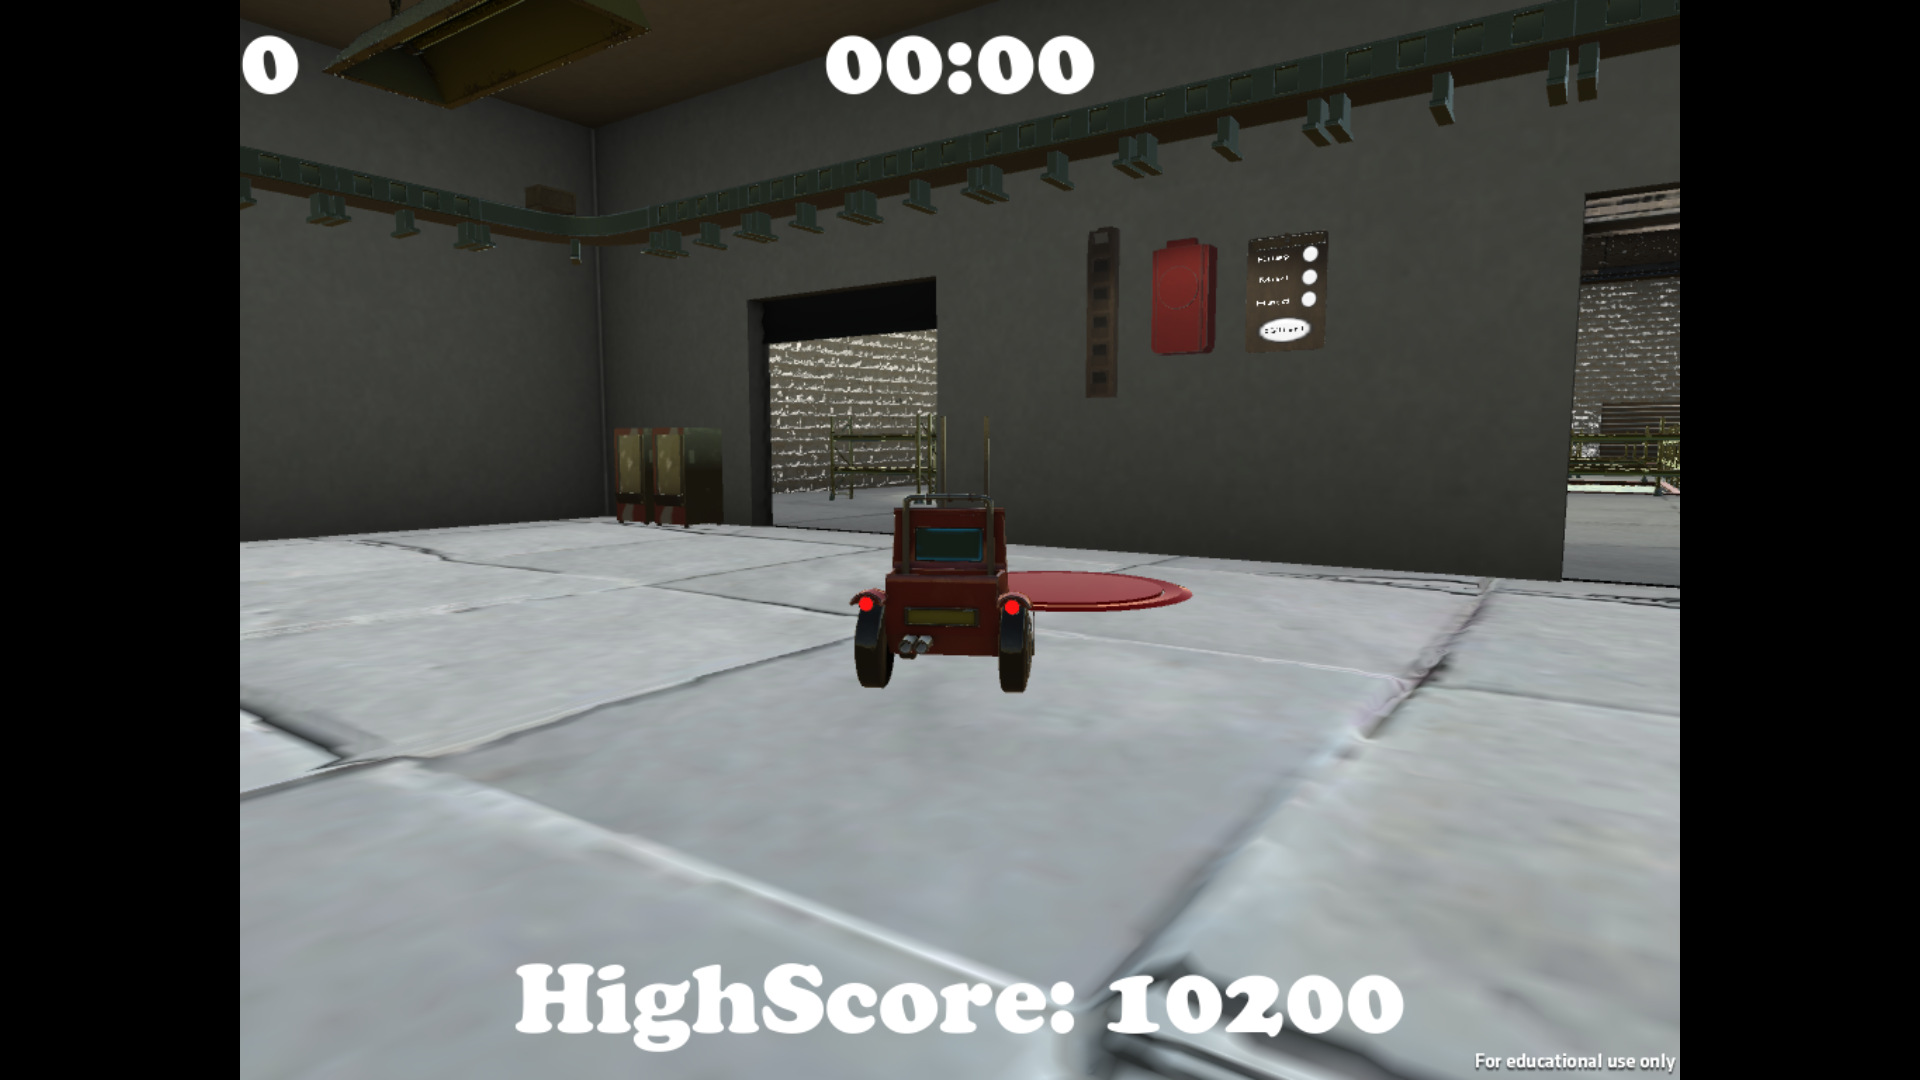
\includegraphics[width=\textwidth]{images/clockInApproach}
\end{figure}
The Clock-In object is how players begin missions within the game; by driving over the red circular activation pad on the ground in the spawn room, players can decide the difficulty level of the mission which affects the number of boxes spawned. 

\begin{figure}[H]
	\caption{Clock In Close-up}
		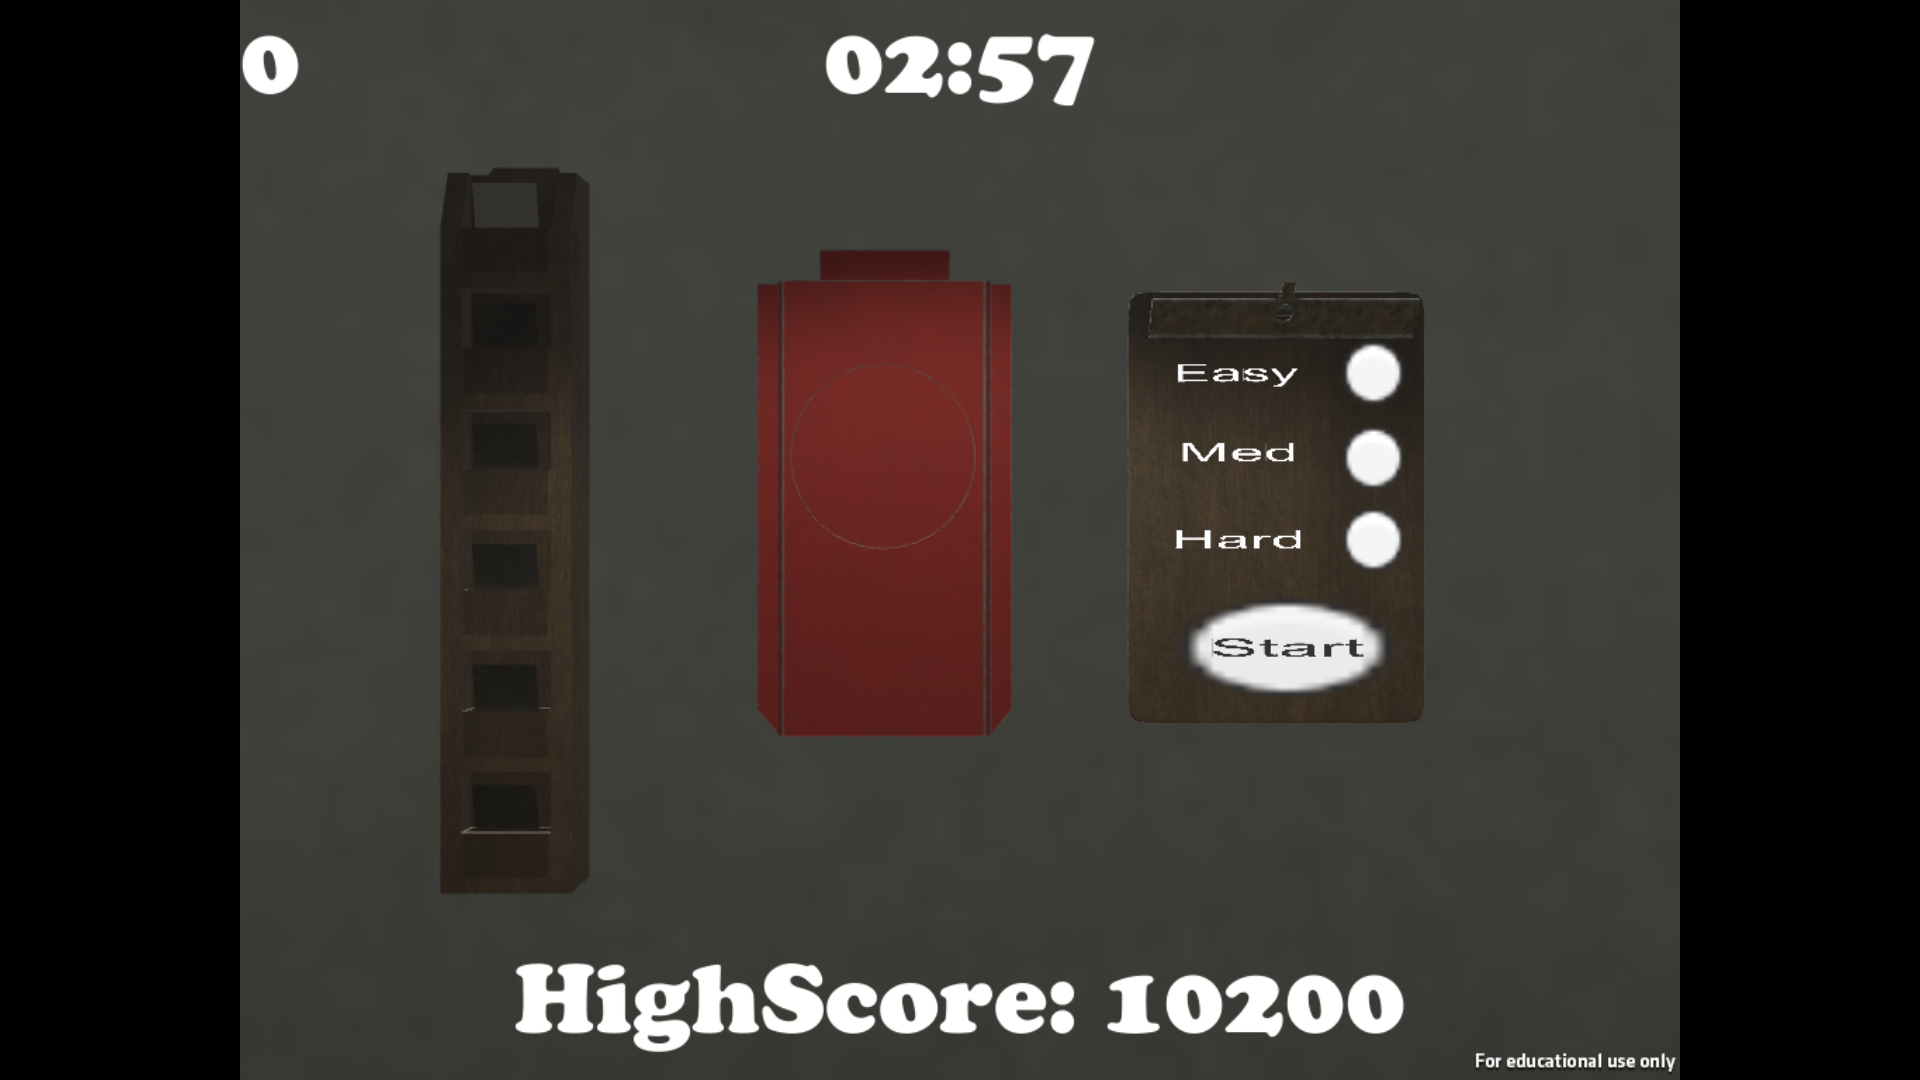
\includegraphics[width=\textwidth]{images/clockInClose}
\end{figure}
A better view of the clock-in model; this clearly shows the in-game user interface with which the players interact to start missions.

\subsubsection{Menu System}
\begin{figure}[H]
	\caption{Pause Screen}
	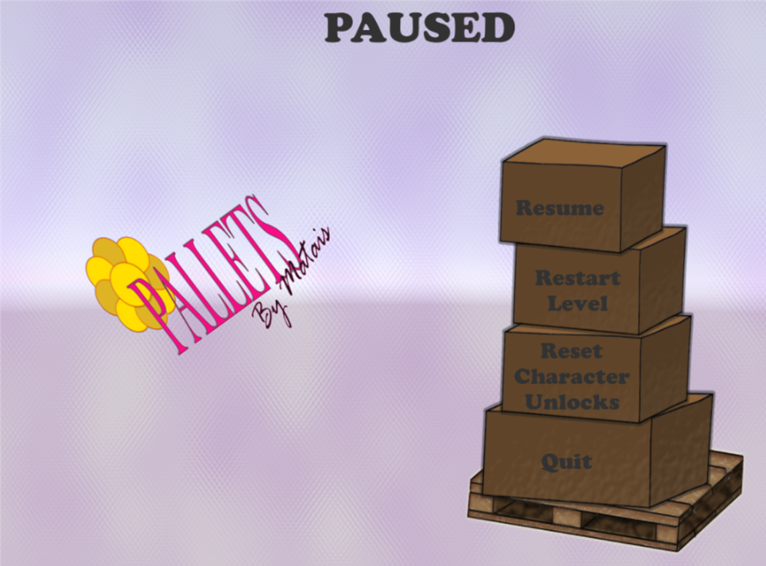
\includegraphics[width=\textwidth]{images/pauseScreen}
\end{figure}
The above image displays the in game pause screen, which has several options the player can interact with. The image shown left of the boxes is chosen randomly from a set, each time the pause screen is opened. 

\begin{figure}[H]
	\caption{Main Menu}
	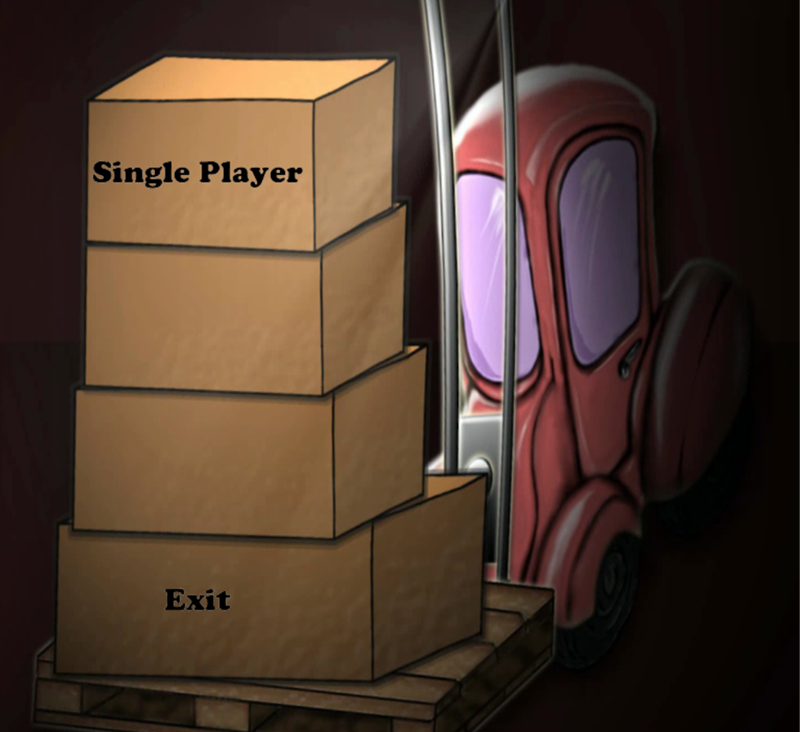
\includegraphics[width=\textwidth]{images/mainMenu}
\end{figure}
The game begins by playing the main menu intro animation; the above forklift drives from screen right into centre screen, with the menu items appearing over the boxes once it stops. Throughout the animation, and whilst in main menu, the game music is playing. 

\begin{figure}[H]
	\caption{Forklift Selection Screen}
	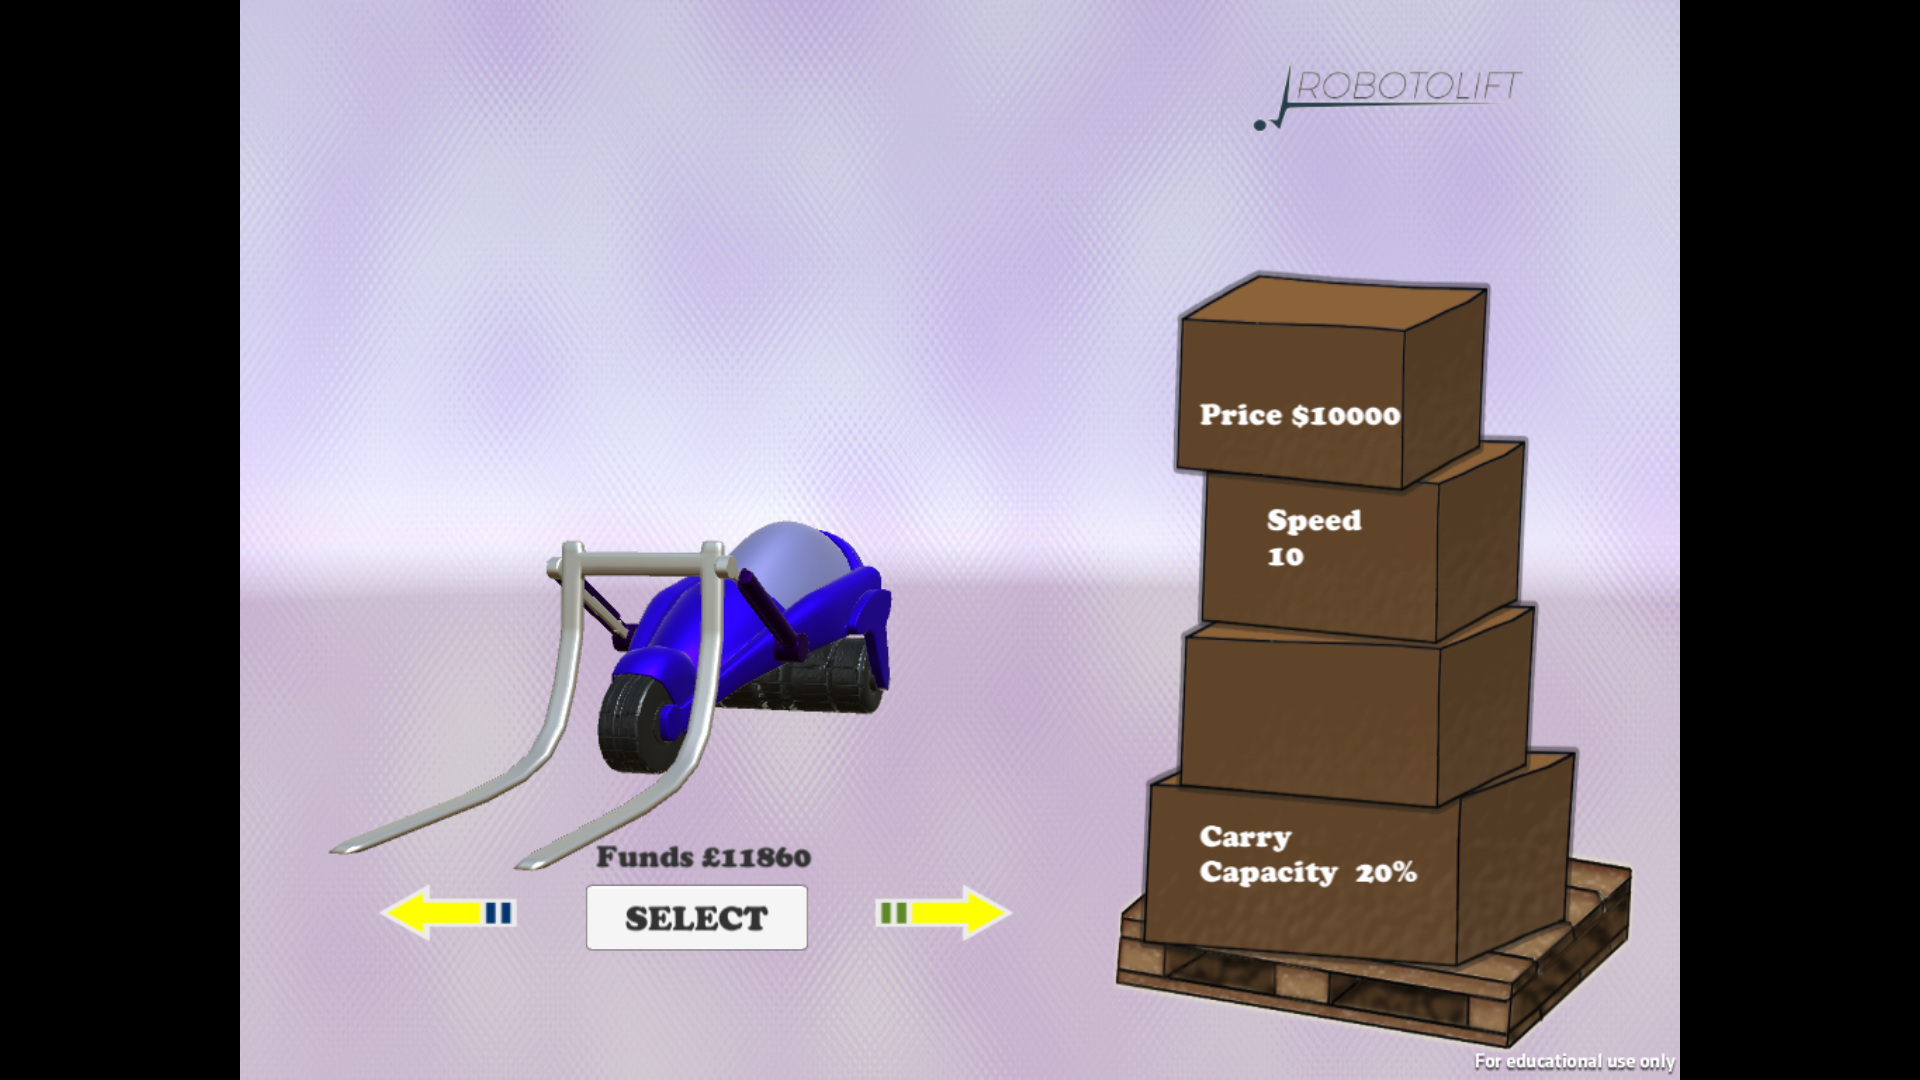
\includegraphics[width=\textwidth]{images/forkliftSelect}
\end{figure}
The forklift selection screen can be opened whilst the player is in the starting room, containing the clock-in object. It shows all four forklifts, their statistics, the players total funds, and allows the player to buy or select the currently displayed forklift. 

\subsubsection{Persistence}
\begin{figure}[H]
	\caption{Persistence Screenshot}
	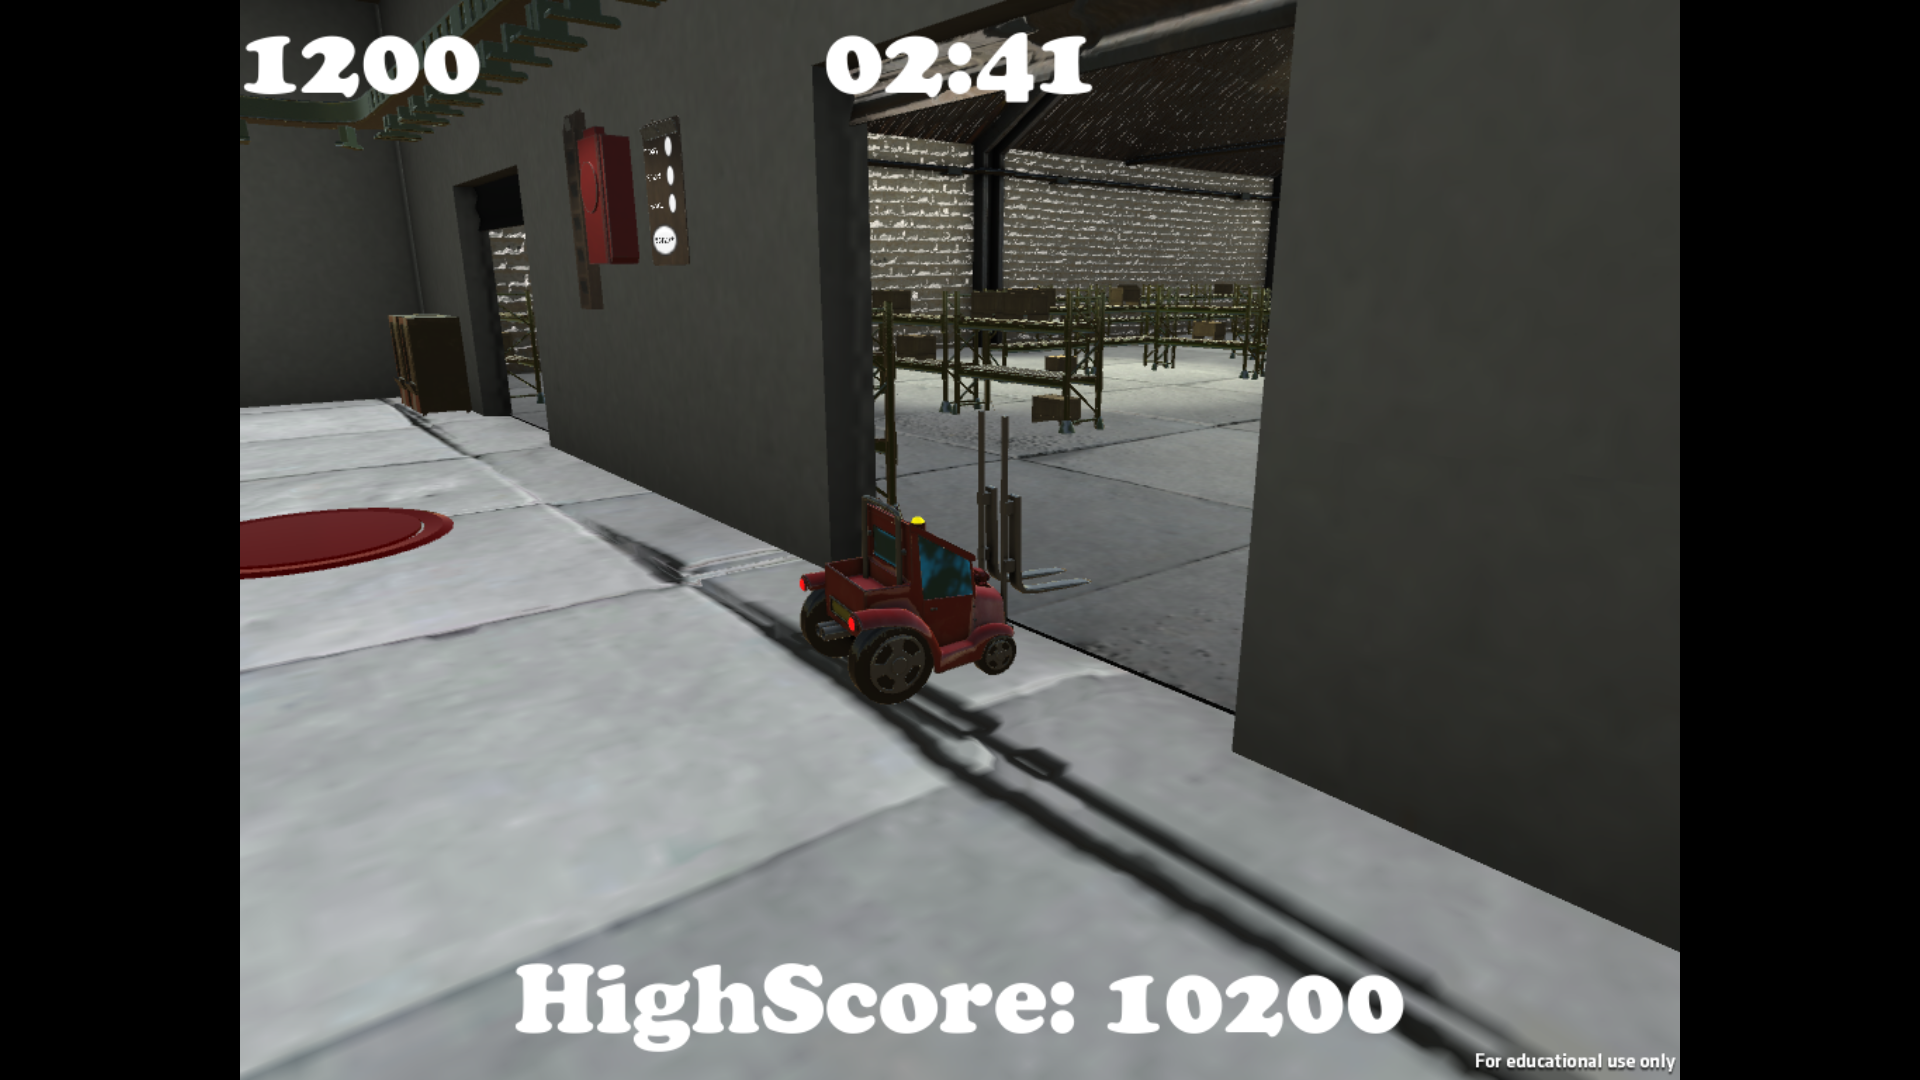
\includegraphics[width=\textwidth]{images/score}
\end{figure}
The above image demonstrates the persistence aim being met; the high score value bottom middle is saved despite closing/reopening the application. As can also be seen in the above forklift selection screen image, the player funds and unlocked forklifts are also maintained over multiple playthroughs after having closed the game.

\subsubsection{Four Forklift Classes}
\begin{figure}[H]
	\caption{Forklift Classes: Redneck (L) \& EZ-Reach (R)}
	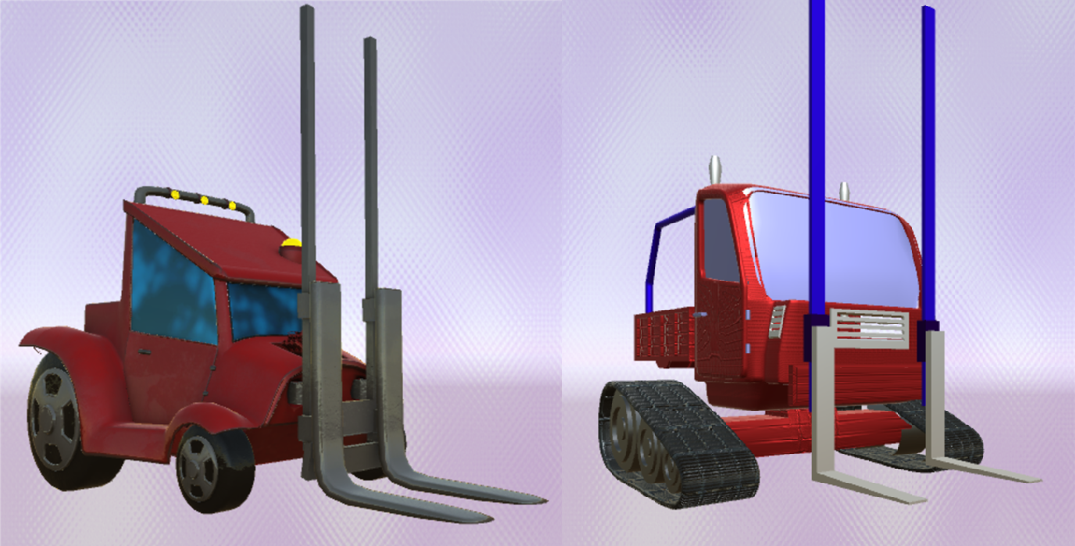
\includegraphics[width=\textwidth]{images/redneckEZ}
\end{figure}
Figure 8 illustrates two of the four forklift classes; Redneck and EZ-Reach models.

\begin{figure}[H]
	\caption{Forklift Classes: DinkyDink (L) \& Robotolift (R)}
	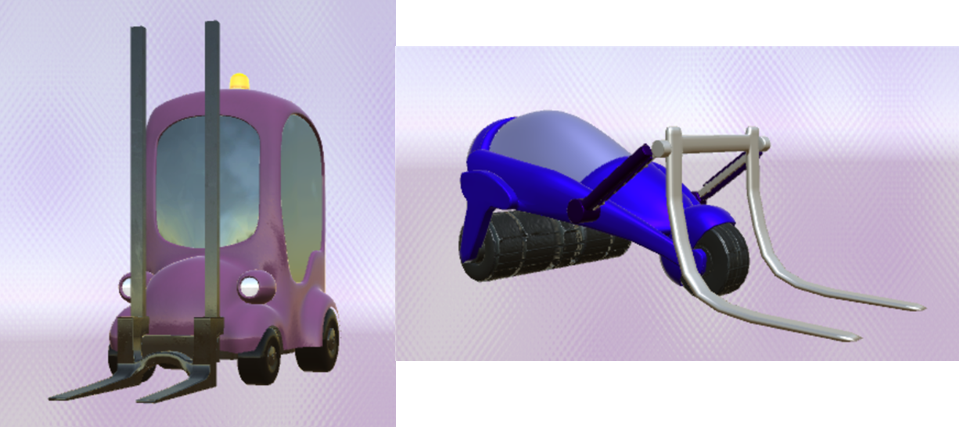
\includegraphics[width=\textwidth]{images/dinkyRobo}
\end{figure}
The above shows the other two forklift classes made for the game; DinkyDink and Robotolift. 


\subsection{Pipeline}
% Describe our working pipeline

After collaboratively working out a plan for features the implementation phase of the project could start. The working pipeline consisted of a similar structure to games development within the industry from concept design, pre-production and onto production. Unfortunately due to the limitations faced during the project, the post-production stage of the development was not fully completed.

\paragraph{Concept Design}

The original concept of the forklift game was conceived before the start of the Group Project in January. This gave the team plenty of time to iron out the designs.

\paragraph{Pre-Production}

During the initial stages of the project, the team had many group meetings for collaborative idea generation. This proved to be a very useful and productive stage of the process. Documentation was created that can be seen in figures \ref{fig:conceptForkSelect}- within Appendix D, this detailed such things as level design, user interface design, mechanics and character design. Code design documentation was also created detailing the classes needed and the required relationships between them.

\paragraph{Production}

Once the design documentation was completed, the production stage could begin. Due to the nature of the tasks, the group could be split into three separate sub-teams to develop artwork, implementation, and sound separately. This model for working although suiting the project proved to be difficult as times as each members work flow relied on each other during the final stages of the project. This seemed to lead into more complex technical issues that were not foreseen in the projects output.

\subsubsection{Artwork}

\subsubsection{Code}

\subsubsection{Sound}

\subsection{Testing}
Types of testing undertaken throughout the project include mostly acceptance criteria testing, with some explorative testing. Testing sessions were planned from project start; aimed to coincide with the completion of major development tasks. However, due to the uncertain nature of the duration of some tasks, testing took on a more ad-hoc nature as the project matured. 

Acceptance criteria testing involves comparing the requirements of a development task with the task deliverable, visually checking that the implementation was correct. Some assets required more testing than others; sound tasks required little testing since after the programming implemented the sounds in game it was a case of hearing if the sound effect played or not, after which it was tweaked to the desired effect. Assets created by artists had to meet the agreed upon standards; naming conventions met, appropriate item groupings and parent/child transform relationships met. This was done by loading the asset into Unity, checking its meta data and viewing the model within the game. Should any criteria not be met, the item was sent back to the owner for updating. 

Explorative testing involves thorough use of the product in as many situations as possible. In this case, that means playing the game through is as many ways as can be thought of. This reveals issues and bugs perhaps previously undiscovered that may have been the result of a knock-on effect after a merge of work, or some change to the game logic, or perhaps an effect that was unaccounted for. While this type of testing was never planned, it was undertaken following acceptance criteria testing for a brief time, and at semi-regular periods throughout the project for a longer duration. Any bugs or issues found through explorative testing were added as issues on Github, where they were later prioritised and included as tasks where appropriate. These issues tended to be minor, requiring only a small amount of time to fix; the final week of development was dedicated to solving these issues. 


\section{Project Management}

\subsection{Approach}
Throughout the project, certain characteristics of the agile methodology were put to use, including:
\begin{itemize}
	\item Close communication and collaboration between all team members throughout, to ensure any problems that arise are dealt with swiftly and with greater efficiency.
	\item Iterative development by means of working in weekly sprints, with clear goals set per sprint, and stand-ups taking place at the beginning of each weekly meeting.
	\item Ensuring flexibility by adjusting task requirements or project goals on the fly. 
\end{itemize}
Adopting the above helped to maintain motivation amongst the group; communication aided in understanding each member's skills and progress, so no one member was left unaware of what others were doing. Working iteratively gave way to quick development cycles since the work done needn't represent a perfect, final product; previous work was improved upon with further tasks, the result of which saw improvements being made more often. Throughout, some tasks' acceptance criteria were adjusted where necessary, and project goals dropped midway, which helped the group to gain focus on the more important, must have, goals.  
\newline
\newline
The MoSCoW method groups all project features into four categories; must have, should have, could have, and won't have. The group's MSCW document proved useful to determine the priority of all features, clearly illustrating the most, and least, important aspects of the product. This was updated after any project goal was re-prioritised, or dropped - such as midway through the project when it was decided that the multiplayer mode and submission to Steam Greenlight were no longer must have goals. This afforded the group a clear view of the latest opinion on each feature. 
\newline
\newline
The project manager/programmer acted as client for this project, which allowed direct communication, quicker decision making, and a technical understanding of the development process. This resulted in saving a lot of time that would otherwise have been spent meeting with an outside client or waiting for decisions to be made, thereby catalysing the development process.
\newline 
\newline
Further to the above, project risks were recorded in the risk register at the start of the project, and kept an eye on throughout. Issues faced later in the project were of a more interpersonal nature, and so dealt with privately on an ad-hoc basis. Backup plans were put in place to cover any work unable to be completed as a result of these issues. 
\subsection{Collaboration}
Various platforms were put in place to allow team members to communicate and collaborate on work with one another. At project start, several pieces of software were available for team use: 
\begin{itemize}
	\item Slack: Work-based messaging software, available on mobile and PC. The team had its own group that allowed users to discuss various topics (art, code, sound, ideas etc) on individual channels. Files were also shared through Slack.  
	\item Google Drive: The primary source of storing all files to do with the project. All members had access, allowing them to make backups of their work. Contains everything from photos of wireframe doodles, project management documents, to assets. Proved invaluable in having one place to store all work.
	\item Github: Used primarily for the scripts created by programmers and sound designer for integrating FMOD into Unity. Allowed completed work to be shared easily and remotely. 
	\item Meistertask: Used to create story cards from tasks assigned to all group members, in tracking the weekly sprint.  
	\item Mural: Allows remote collaboration via an online drawing/planning tool. Allowed the team to create storyboards and share ideas throughout the week. 
\end{itemize}

A few weeks into the project, however, saw the disuse of both Meistertask and Mural; it was evident that there were too many platforms for team members to record their ideas and view details of current or upcoming tasks. Following similar feedback from the team, task details and storyboards were moved to Google Drive, leaving only two or three places that team members need keep up to date with. This proved more effective, allowing the team to focus on development rather than admin. In order to encourage regular communication throughout the team, the project manager routinely wrote into the group chat and paid attention to the replies; should any member not be responsive throughout the week, they would receive a personal message inquiring about their progress. 

As regards communication with module staff, the project manager and lead programmer attended weekly meetings with the group supervisor, to keep him updated on progress or issues for that week. The module leader was consulted on a few occasions, regarding setting up a git server for the team, and further consultation on issues. 

\subsection{Schedule} 
\begin{figure}[H]
	\caption{Original Timeline Plan}
	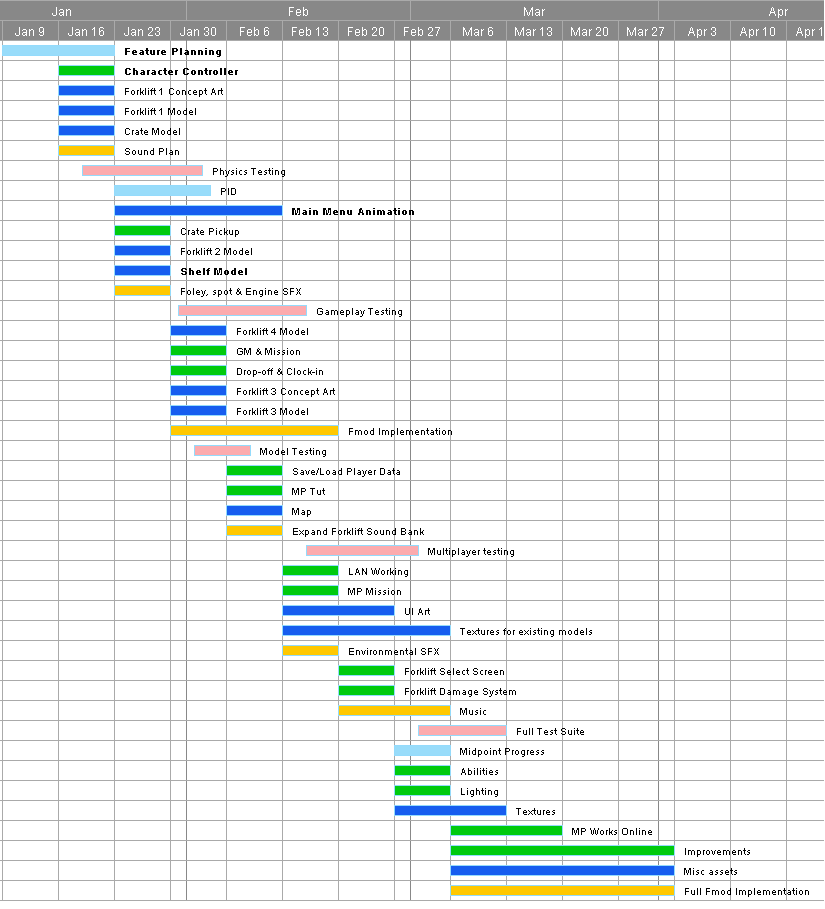
\includegraphics[width=\textwidth]{images/ganttChart}
\end{figure}
The above figure illustrates the original gantt chart included in the PID, as was planned prior to project kick-off. 
\begin{figure}[H]
	\caption{Living Timeline}
	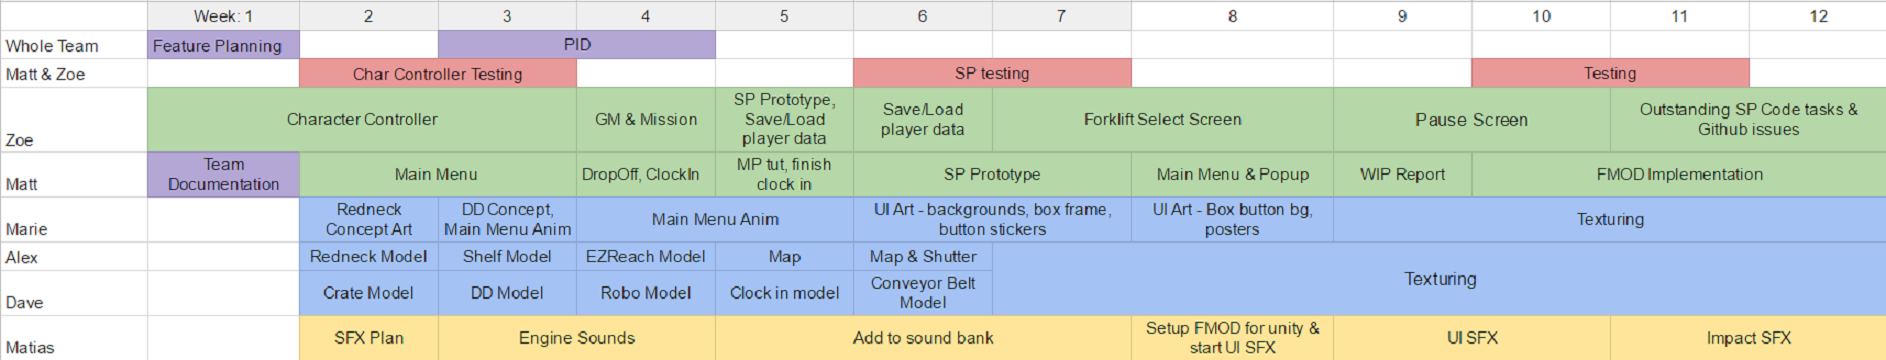
\includegraphics[scale=0.4]{images/livingTimeline}
\end{figure}
The above figure displays the actual timeline, which was kept updated throughout the project. 

As is evident by comparing the above images of the teams predicted and actual progress, changes were made throughout the project. These changes were a necessity brought about largely by the difference between the projected and resulting time requirements of tasks. In keeping with Agile methodology, more time was allocated where necessary to certain tasks, thereby pushing back others. The original plan was useful in keeping goals in mind, whilst allowing a fluidity in the arrangement of tasks. 

\section{Conclusion}

\newpage
\clearpage

\section{Appendix A}

\section{Appendix B}

\section{Appendix C}
\section{Appendix D}

\figuremacro{h}{conceptForkSelect}{Pre-production }{- concept design for forklift selection scene.}{1.0}
\figuremacro{h}{overheadMapLayout}{Pre-production }{- original multiplayer map design.}{1.0}


\end{document}